\chapter{MIMD and SIMD Tree Traversals}
\section{Overview}

For a full language, statically identified parallelization opportunities still require an efficient runtime implementation that exploits them. In this section, we show how to exploit the logical concurrency identified within a tree traversal to optimize for the architectural properties of two types of hardware platforms: MIMD (e.g., multicore) and SIMD (e.g., sub-word SIMD and GPU) hardware. For both types of platforms, we optimize the schedule within a traversal and the data representation. We innovate upon known techniques in several ways:

\begin{enumerate}
\item \textbf{Semi-static work stealing for MIMD:} MIMD traversals should be optimized for low overheads, load balancing, and locality. Existing techniques such as work stealing provide spatial locality and, with tiling, low overheads. However, dynamic load balancing within a traversal leads to poor temporal locality across traversals. The processor a node is assigned to in one traversal may not be the same one in a subsequent traversal, and as the number of processors increases, the probability of assigning to a different one increases. Our solution dynamically load balances one traversal and, due to similarities across traversals, successfully reuses it.
\item \textbf{Clustering traversals for SIMD:}  SIMD evaluation is sensitive to divergence across parallel tasks in instruction selection. Visits to different types of tree nodes yield different instruction streams, so na\i{v}e vectorization fails for webpages due to their visual variety. Our insight is that similar nodes can be semi-statically identified. Thus \emph{clustered} nodes will be grouped in the data representation and run in SIMD at runtime.
\item \textbf{Automatically staged parallel memory allocation to efficiently combine SIMD layout and SIMD rendering:} We optimized the schedule of memory allocations in the layout computation into an efficient parallel prefix sum. Otherwise, parallel dynamic memory allocation requests would contend over the free memory buffer and void GPU performance benefits. We automated the optimization by reducing the scheduling problem to attribute grammar scheduling and automatically performing the reduction through macro expansion.
\end{enumerate}

Our techniques are important and general. They overcame bottlenecks preventing seeing any speedup from parallel evaluation for webpage layout and data visualization. Notably, they are generic to computations over trees, not just layout. An important question going forward is how to combine them as, in principle, they are complementary.

\section{MIMD: Semi-static work stealing}
\subsection{Scheduling}
\subsection{Data representation}
\subsection{Evaluation}


\section{SIMD Background: Level-Synchronous Breadth-First Tree Traversal}
The common baseline for our two SIMD optimizations is to implement parallel preorder and postorder tree traversals as level-synchronous breadth-first parallel tree traversals. Reps first suggested such an approach to parallel attribute grammar evaluation [[CITE]], but did not implement it. Performance bottlenecks led to us deviate from the core representation used by more recent data parallel languages such as NESL [[CITE]] and Data Parallel Haskell [[CITE]]. We discuss our two innovations in the next subsections, but first overview the baseline technique established by existing work.

\newsavebox{\bfsVisitor}
\begin{lrbox}{\bfsVisitor}% Store first listing
\begin{lstlisting}[mathescape,language=C++,morekeywords={spawn,join,reverse,parallel_for}]
void parPre(void (*visit)(Prod &), List<List<Prod>>  &levels) {
  for (List<Prod> level in levels)
  	parallel_for (Prod p in level)
		visit(p)
}
void parPost(void (*visit)(Prod &), List<List<Prod>>  &levels) {
  for (Array<Prod> level in levels.reverse())
  	parallel_for (Prod p in level)
		visit(p)
}\end{lstlisting}
\end{lrbox}

\begin{figure}
\subfloat[\textbf{Level-synchronous Breadth-First Traversal}]{\label{fig:bfstraversal:code}  \usebox{\bfsVisitor}  } \\
\subfloat[\textbf{Logical Tree}]{\label{fig:bfstraversal:replog} 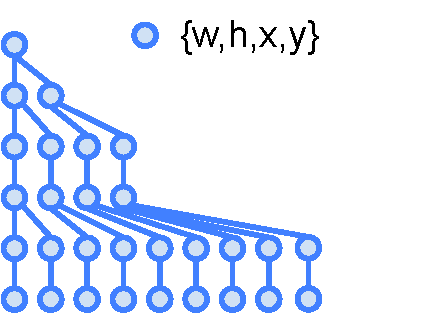
\includegraphics[trim=0 0 0 0,clip,width=0.3\columnwidth]{chapter6/bfslayouttree} } 
 \subfloat[\textbf{Tree Representation}]{\label{fig:bfstraversal:repmem}  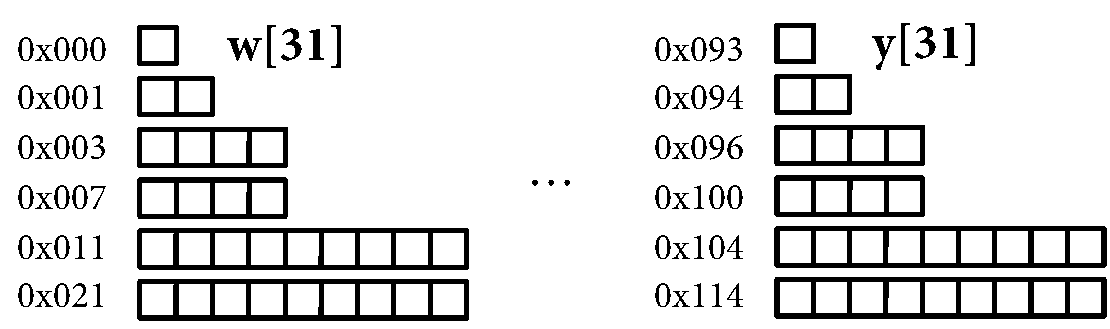
\includegraphics[trim=0 0 0 0,clip,width=0.6\columnwidth]{chapter6/bfslayoutmem} } 
\caption{\textbf{SIMD tree traversal as level-synchronous breadth-first iteration with corresponding structure-split data representation.}}
\label{fig:bfstraversal}
\end{figure}

The na\i{v}e tree traversal schedule is to sequentially iterate one level of the tree at a time and  traverse the nodes of a level in parallel. A parallel preorder traversal starts on the root node's level and then proceeds downwards, while a postorder traversal starts on the tree fringe and moves upwards (Figure~\ref{fig:bfstraversal}~\ref{fig:bfstraversal:code}). Our MIMD implementation, in contrast, allows one processor to compute on a different tree level than another active processor. In data visualizations, we empirically observed that most of the nodes on a level will dispatch to the same layout instructions, so our na\i{v}e traversal schedule avoids instruction divergence.

The level-synchronous traversal pattern eliminates many divergent memory accesses by using a corresponding data representation. Adjacent nodes in the schedule are collocated in in memory. Furthermore, individual node attributes are stored in \emph{column} order through a array-of-structure to structure-of-array conversion. The conversion collocates individual attributes, such as the width attribute of one node being stored next to the width attribute of the node's sibling (Figure~\ref{fig:bfstraversal:repmem}). The index of a node in a breadth-first traversal of the tree is used to perform a lookup in any of the attribute arrays. The benefit this encoding is that, during SIMD  layout of several adjacent nodes, reads and writes are coalesced into  bulk reads and writes. For example, if a layout pass adds a node's padding to its width, several contiguous paddings and several contiguous widths will be read, and the sum will be stored with a contiguous write. Such optimizations are crucial because the penalty of non-coalesced access is high and, for layout, relatively few computations occur between the reads and writes.

Full implementation of the data representation poses several subtleties. 
\begin{itemize}
\item \textbf{Level representation.} To eliminate traversal overhead, a summary provides the index of the first and last node on each level of a tree. Such a summary provides  data range information for launching the parallel kernels that evaluate the nodes of a level as well as the information for how to proceed to the next level.
\item \textbf{Edge representation.} A node may need multiple named lists of children, such as an HTML table with a header, footer, and an arbitrary number of rows. We encode the table's edges as 3 global arrays of offsets: header, footer, and first-row. To support iterating across rows, we also introduce a 4th array to encode whether a node is the last sibling. Thus, any named edge introduces a global array for the offset of the pointed-to node, and for iteration, a shared global array reporting whether a node at a particular index is the end of a list.
\item \textbf{Memory compression.} Allocating an array the size of the tree for every type of node attribute wastes memory. We instead statically compute the maximum number of attributes required for any type of node, allocate an array for each one, and map the attributes of different types of nodes into different arrays. For example, in a language of HBox nodes as Circle nodes who have attributes 'r' and 'angle', 4 arrays will be allocated. The HBox requires an array for each of the attributes 'w', 'h', 'x', and 'y' while the Circle nodes only require two arrays. Each node has one type, and if that that type is HBox, the node's entry in the first array will contain the 'w' attribute. If the node has type Circle, the node's entry in the first entry will contain the 'r' attribute.
\item \textbf{Tiling.} Local structural mutations to a tree such as adding or removing nodes should not force global modifications. As most SIMD hardware has limited vector lengths (e.g., 32 elements wide), we split our representation into blocks. Adding nodes may require allocation of a new block and reorganization of the old and new block. Likewise, after successive additions or deletions, the overall structure may need to be compacted. Such techniques are standard for file systems, garbage collectors, and databases.
\end{itemize}


In summary, our basic SIMD tree traversal schedule and data representation descend from the approach of NESL [[CITE]] and Data Parallel Haskell [[CITE]]. Previous work shows how to generically convert a tree of structures into a structure of arrays. Those approaches do not support statically unbounded nesting depth (i.e., tree depth), but our system supports arbitrary tree depth because our transformation is not as generic.  

A key property of all of our systems, however, is that the structure of the tree is fixed prior to the traversals.  In contrast, for example, parallel breadth-first traversals of graphs will dynamically find a minimum spanning tree [[CITE]]. Such dynamic alternatives incur unnecessary overheads when performing a sequence of traversals and sacrifice memory coalescing opportunities. Layout is often a repetitive process, whether due to multiple tree traversals for one invocation or an animation incurring multiple invocations, so costs in creating an optimized data representation and schedule are worth paying.

\section{Input-dependent Clustering for SIMD Evaluation}


Once the tree is available, we automatically optimize the schedule for traversing a tree level in a way that avoids instruction divergence. Our insight is that we can cluster tasks (nodes) based on node attributes that influence control flow. We match the data layout to the new schedule, and optimize the clustering process to prevent the planning overhead to outweigh its benefit. The overall optimization can be thought of an extension to loop unswitching where the predicate is input-dependent and a sorting prepass guarantees that subintervals will branch identically.

\begin{figure}
\subfloat{  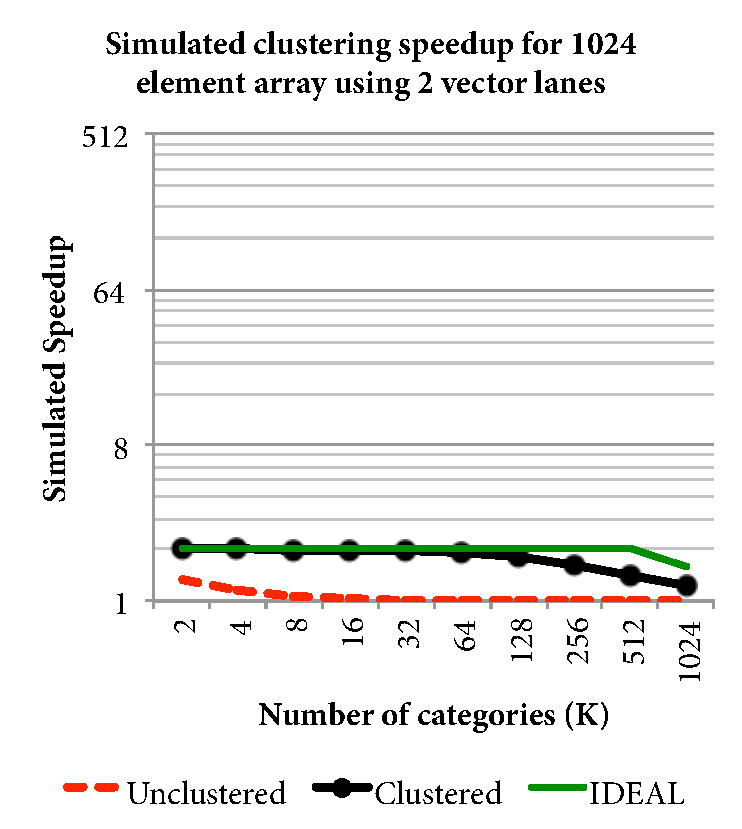
\includegraphics[trim=0 0 0 0,clip,width=0.32\columnwidth]{chapter6/simulatedclusteringspeedup/simulatedclusteringspeedup-1} }
\subfloat{  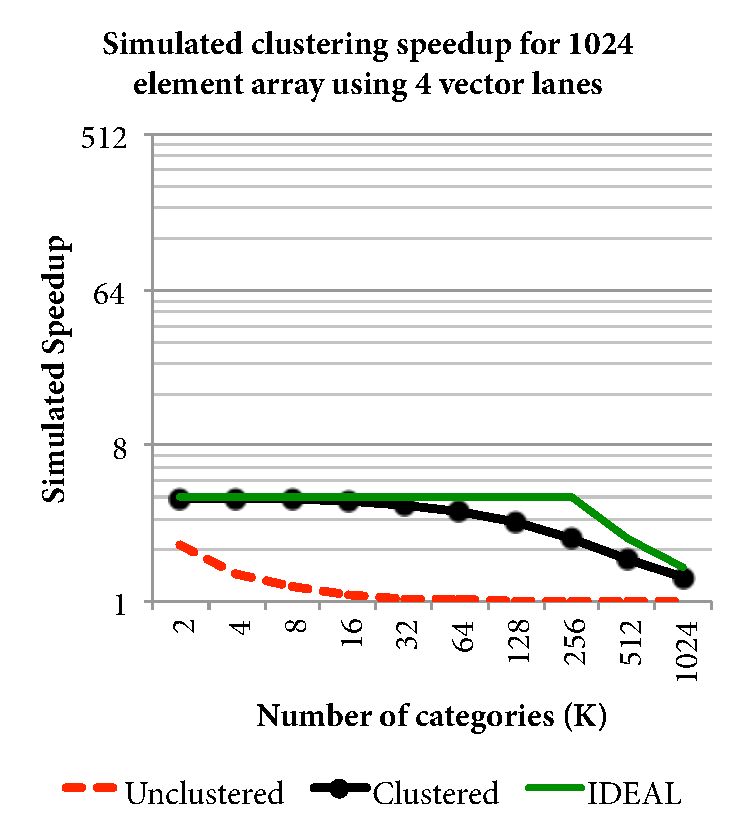
\includegraphics[trim=0 0 0 0,clip,width=0.32\columnwidth]{chapter6/simulatedclusteringspeedup/simulatedclusteringspeedup-2} }
\subfloat{  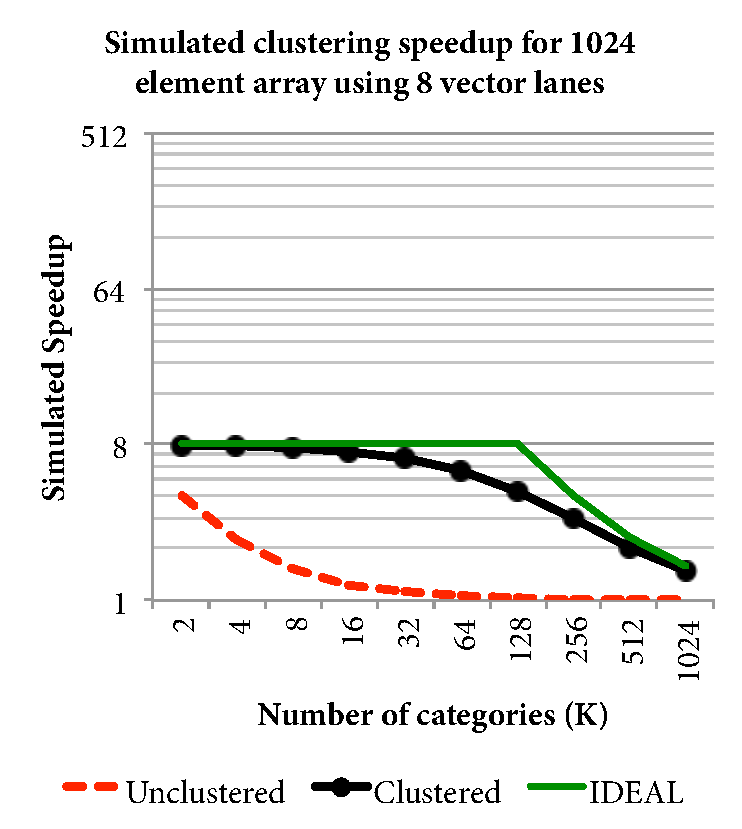
\includegraphics[trim=0 0 0 0,clip,width=0.32\columnwidth]{chapter6/simulatedclusteringspeedup/simulatedclusteringspeedup-3} } \\
\subfloat{  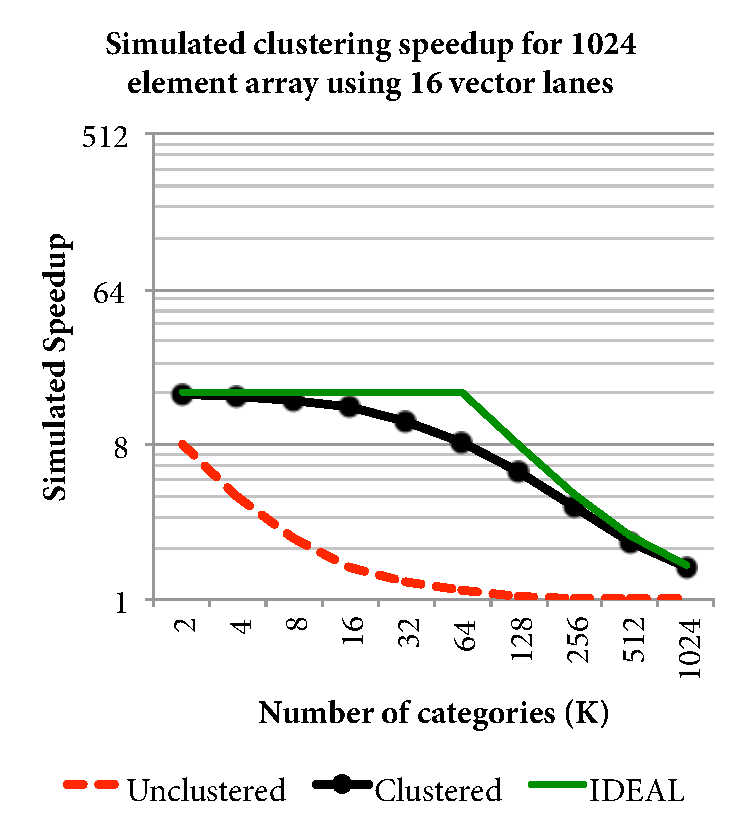
\includegraphics[trim=0 0 0 0,clip,width=0.32\columnwidth]{chapter6/simulatedclusteringspeedup/simulatedclusteringspeedup-4} }
\subfloat{  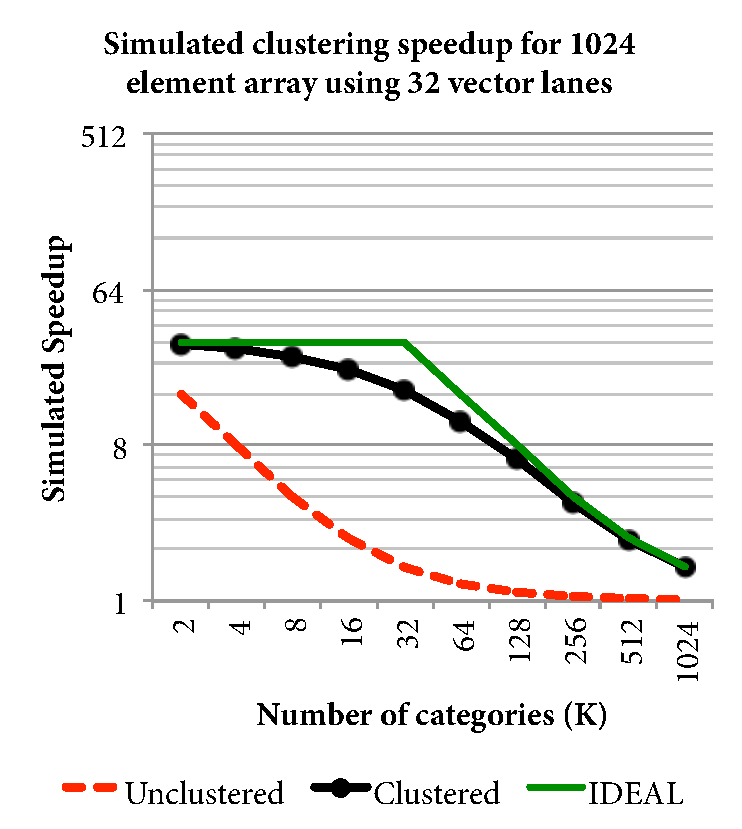
\includegraphics[trim=0 0 0 0,clip,width=0.32\columnwidth]{chapter6/simulatedclusteringspeedup/simulatedclusteringspeedup-5} }
\subfloat{  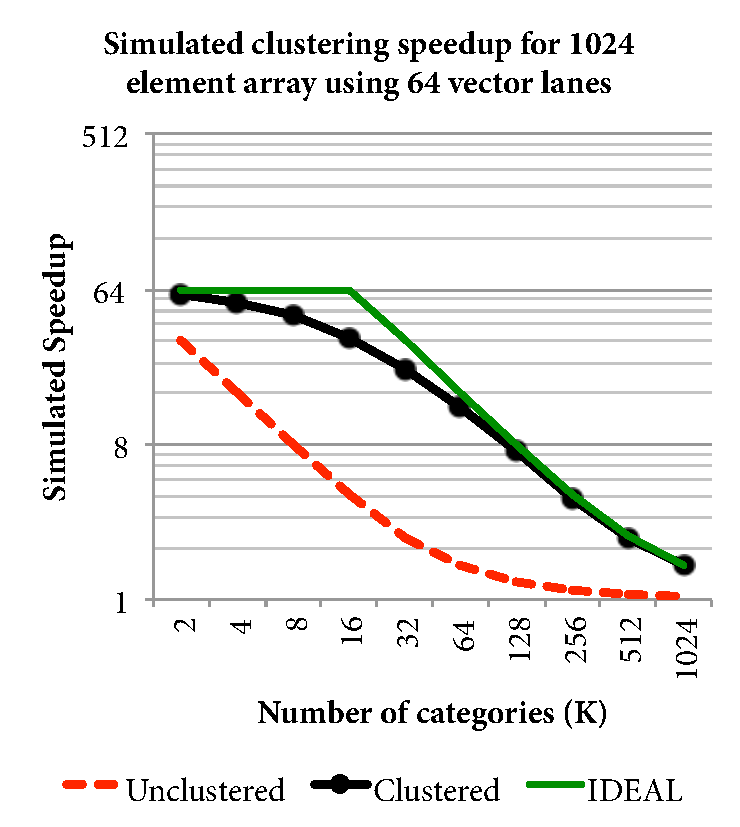
\includegraphics[trim=0 0 0 0,clip,width=0.32\columnwidth]{chapter6/simulatedclusteringspeedup/simulatedclusteringspeedup-6} } \\
\subfloat{  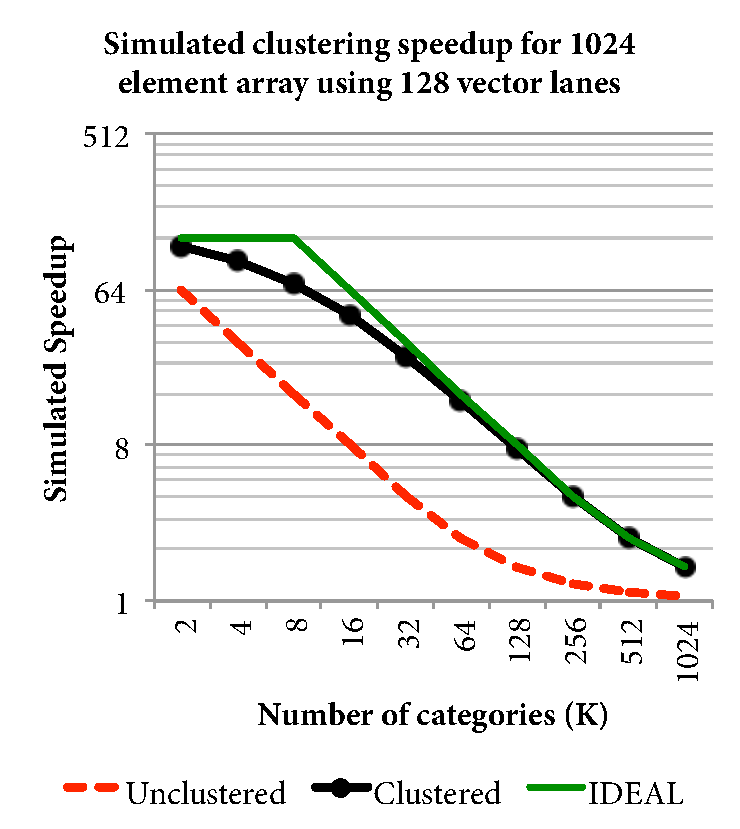
\includegraphics[trim=0 0 0 0,clip,width=0.32\columnwidth]{chapter6/simulatedclusteringspeedup/simulatedclusteringspeedup-7} }
\subfloat{  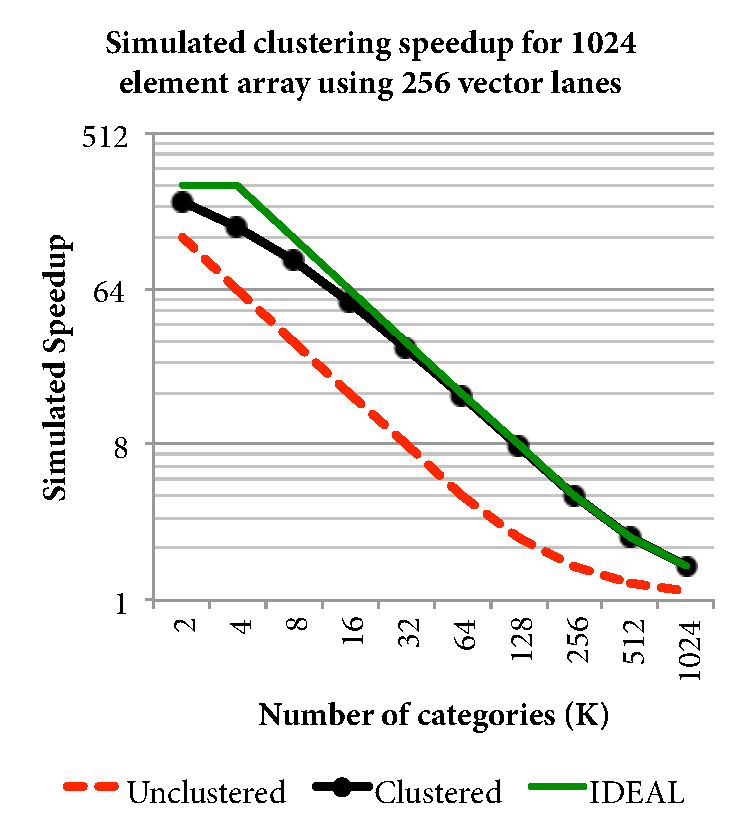
\includegraphics[trim=0 0 0 0,clip,width=0.32\columnwidth]{chapter6/simulatedclusteringspeedup/simulatedclusteringspeedup-8} }
\subfloat{  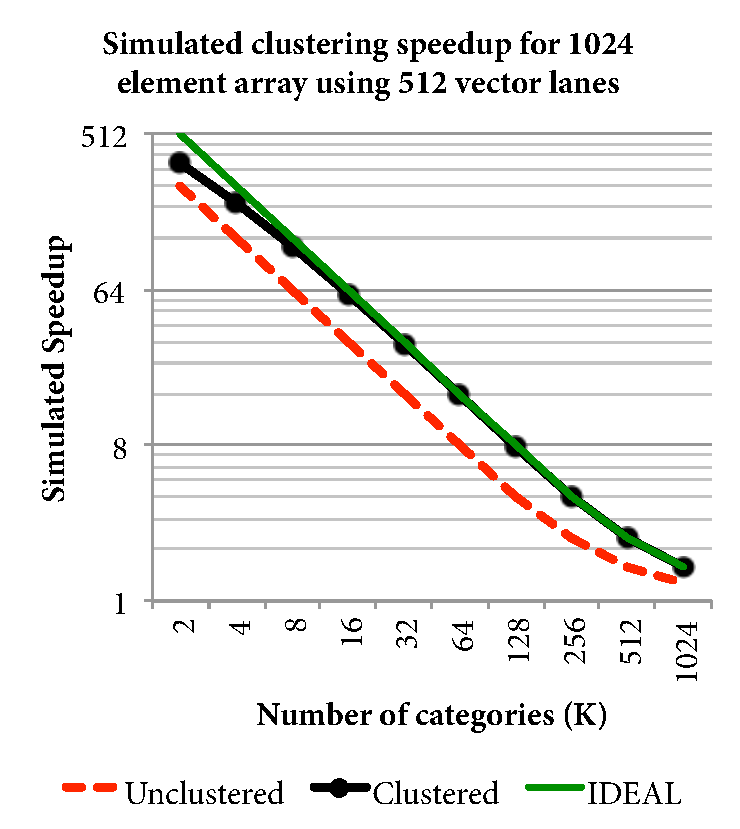
\includegraphics[trim=0 0 0 0,clip,width=0.32\columnwidth]{chapter6/simulatedclusteringspeedup/simulatedclusteringspeedup-9} } \\
\caption{\textbf{blah}}
\label{fig:simulatedclusteringspeedup}
\end{figure}





\subsection{The Problem}
The problem we address stems from layout being a computation where the instructions for each node are heavily input dependent. The intuition can be seen in contrasting the visual appearance of a webpage vs. a data visualization. Different parts of a webpage look quite different from one another, which suggests sensitivity to values in the input tree, while a visualization looks self-similar and thus does not use widely different instructions for different nodes.  For an example of divergence, an HBox's width is the sum of its children widths, while a VBox's is their maximum. The visit to a node (Figure~\ref{fig:compiled}) will diverge in instruction selection based on the node type.  

We ran a simulation to measure the performance cost of the divergence. Assuming a uniform distribution of types of nodes in a level, as the number of types of nodes go up ($K$), the probability that all of the nodes in a group share the same instructions drops exponentially. Figure~\ref{fig:simulatedclusteringspeedup} shows the simulated speedup for SIMD evaluation over a tree level of 1024 nodes on computer architectures with varying SIMD lengths. The x axis of each chart represents the number of types and the y axis is the speedup. As the number of choices increase, the benefit of the na\i{v}e breadth-first schedule (red line) decreases. It is far from the ideal speedup, which we estimated as a function of the SIMD length of the architecture (maximal parallel speedup, contributing the horizontal portion of the green lines) and the expected number of different categories (mandatory divergences, contributing the diagonal portion). 

\subsection{Code Clustering}
Our solution is to cluster nodes of a level based on the values of attributes that influence the flow of control. SIMD evaluation of the nodes in a cluster will be free of instruction divergence. Furthermore, by changing the data representation to match the clustered schedule, memory accesses will also be coalesced. We first focus on applying the clustering transformation to the code.



\newsavebox{\bfsClusteredVisitor}
\begin{lrbox}{\bfsClusteredVisitor}% Store first listing
\begin{lstlisting}[mathescape,language=C++,morekeywords={spawn,join,reverse,parallel_for}]
void parPreClustered(void (*visit)(Prod &), List<List<Array<Prod>>>  &levels) {
  for (List<Prod> level in levels)
  	for (Array<Prod> cluster in level)
  		parallel_for (Prod p in cluster)
			visit(p)
}
\end{lstlisting}
\end{lrbox}

\begin{figure}
 \usebox{\bfsClusteredVisitor}  
\caption{\textbf{Clustered parallel preorder traversal.}}
\label{fig:clusteredeval}
\end{figure}


\newsavebox{\clusterUnswitchA}
\begin{lrbox}{\clusterUnswitchA}% Store first listing
\begin{lstlisting}[mathescape]
Prod firstProd = cluster[0]
parallel_for (prod in Cluster) {
  switch (firstProd.type) {
    case S $\rightarrow$ HBOX:  break;
    case HBOX $\rightarrow$ $\epsilon$:
      HBOX.w = input(); 
      HBOX.h = input(); 
      break;
    case HBOX $\rightarrow$ HBOX$_1$ HBOX$_2$:
      HBOX$_0$.w = HBOX$_1$.w + HBOX$_2$.w;
      HBOX$_0$.h = MAX(HBOX$_1$.h, HBOX$_2$.h);
      break;
  }
 }
\end{lstlisting}
\end{lrbox}

\newsavebox{\clusterUnswitchB}
\begin{lrbox}{\clusterUnswitchB}% Store first listing
\begin{lstlisting}[mathescape]
Prod firstProd = cluster[0]
  switch (firstProd.type) {
    case S $\rightarrow$ HBOX:  break;
    case HBOX $\rightarrow$ $\epsilon$:
      parallel_for (prod in Cluster) {
          HBOX.w = input(); 
          HBOX.h = input();
     }
      break;
    case HBOX $\rightarrow$ HBOX$_1$ HBOX$_2$:
      parallel_for (prod in Cluster) {
        HBOX$_0$.w = HBOX$_1$.w + HBOX$_2$.w;
        HBOX$_0$.h = MAX(HBOX$_1$.h, HBOX$_2$.h);
      }
      break;
  }
 }
\end{lstlisting}
\end{lrbox}



\begin{figure}
\subfloat[\textbf{Clustered dispatch.}]{ \usebox{\clusterUnswitchA} } 
\subfloat[\textbf{Unswitched dispatch}.]{\usebox{\clusterUnswitchB} } 
\caption{\textbf{Loop transformations to exploit clustering for vectorization.}}
\label{fig:clusteringunswitching}
\end{figure}


Figure~\ref{fig:clusteredeval} shows the clustered evaluation variant of the MIMD $parPre$ traversal of Figure~\ref{fig:hboxall}. The traversal schedule is different because the order is based on the clustering rather than breadth-first index. Changing the order is safe because the original loop was parallel with no dependencies between elements.  Computing over clusters guarantees that all calls to a visit dispatch function in the parallel inner loop (e.g., of $visit1$) will branch to the same switch statement case. This modified schedule avoids instruction divergence. 

Our loop transformation can be understood as a use of loop unswitching, which is a common transformation for improving parallelization. Loop unswitching lifts a conditional out of a loop by duplicating the  loop inside of both cases of the conditional. Clustering establishes the invariant of being able to inspect the first item of a collection sufficing for performing unswitching for a loop over all of the items. Figure~\ref{fig:clusteringunswitching} separates our transformation of $visit1$ (Figure \ref{fig:hboxall}) into using the same exemplar for the dispatch and then loop unswitching.

Clustering is with respect to input attributes that influence control flow, which may be more than the node type. For example, in our parallelization of the C3 layout engine, we found that the engine author combined the logic of multiple box types into one visit function because the variants shared a lot of code. He instead used multiple node flags to guide instruction selection. Both the node type and various other node attributes influenced control flow, and therefore our clustering condition was on whether they were all equal. Using all of the attributes led to too granular of a clustering condition, so we manually tuned the choice of attributes.

\subsection{Data Clustering}
The data representation should be modified to match the clustering order. The benefit is coalesced memory accesses, but overhead costs in performing the clustering should be considered.

Our algorithm matches the data representation order to the schedule by placing nodes of a cluster into the same contiguous array. Parallel reads and are coalesced, such as the inspection of the node type for the visit dispatch. Parallel writes are likewise coalesced.

Reordering data is expensive as all of the data is moved. In the case of our data visualization system, we can avoid the cost because the data is preprocessed on our server. For webpage layout, the client performs clustering, which we optimize enough such that the cost is outweighed by the subsequent performance improvements.

We optimize reordering with a simple parallel two-pass technique. The first pass traverses each level in parallel to compute the cluster for each node and tabulate the cluster sizes for each tree level. The second pass again traverses each level in parallel, and as each node is traversed, copies it into the next free slot of the appropriate cluster. Even finer-grained parallelization is possible, but this algorithm was sufficient for lowering reordering costs enough to be amortized.

\subsection{Nested Clustering}
Clustering can also be used to address divergences induced by computations over neighboring nodes. They avoidable irregularities can take several forms:

\begin{itemize}
\item \textbf{Branches.} For the case of webpage layout, we saw cases where attributes of the parent node or children node influence instruction selection, such as whether to include a child node in a width computation. The properties can be included in the clustering condition to eliminate the corresponding instruction divergences. 

\item \textbf{Load imbalance in loops.} One node may have no children while another may have many. If the layout computation involves a loop, SIMD evaluation will perform the two loops in lock-step. Thus, as the nodes have different amounts of children, the SIMD lanes devoted to the first child will not be utilized: this is a load balancing problem. The number of children can be included in the clustering condition to eliminate load imbalance.

\item \textbf{Random memory access in loops.} A further issue with lock-step loops over child nodes is memory divergence. A breadth-first layout would provide strided memory access, but if each level is clustered, the locations of a node's children may be random without further aid. We found a \emph{nested} solution where \emph{subtrees} are assigned to clusters. Instead of just associating nodes of a level with a cluster, our algorithm then treats the nodes of a cluster as roots. It recursively expands a subtree such that all of the cluster nodes share it (with respect to the attributes influencing control flow). The data layout follows the nested clustering, so parallel memory accesses to the children of nodes will be coalesced. 
\end{itemize}

Each of these clusterings introduce an invariant for a cluster for optimizing performance within that cluster. However, the clustering condition is more discriminating.  Cluster sizes may decrease, which would  significantly decrease  performance if cluster size shrinks below vector length size. Our evaluation explores these options in practice.


\newsavebox{\stagedAllocFull}
\begin{lrbox}{\stagedAllocFull}% Store first listing
\begin{lstlisting}[mathescape]
float *drawCircle (float x, float y, float radius) {
  float *buffer = malloc( (2 * sizeof(float) ) * round(radius))
  for (int i = 0; i < round(radius); i++) {
    buffer[2 * i] = x + cos(i * PI/radius);
    buffer[2 * i + i] = y + sin(i * PI/radius);
  }
  return buffer;
}
\end{lstlisting}
\end{lrbox}

\newsavebox{\stagedAllocAlloc}
\begin{lrbox}{\stagedAllocAlloc}% Store first listing
\begin{lstlisting}[mathescape]
int allocCircle (float x, float y, float radius) {
  return round(radius);
}
\end{lstlisting}
\end{lrbox}


\newsavebox{\stagedAllocRender}
\begin{lrbox}{\stagedAllocRender}% Store first listing
\begin{lstlisting}[mathescape]
int fillCircle(float x, float y, float radius, float *buffer) {
  for (int i = 0; i < round(radius); i++) {
    buffer[2 * i] = x + cos(i * PI/radius);
    buffer[2 * i + i] = y + sin(i * PI/radius);
  }	
  return 0;
}
\end{lstlisting}
\end{lrbox}


\begin{figure}
\subfloat[\textbf{Na\i{v}e drawing primitive .}]{\label{fig:stagedalloc:original} \usebox{\stagedAllocFull} }  \\
\subfloat[\textbf{Allocation phase of drawing}.]{\label{fig:stagedalloc:alloc} \usebox{\stagedAllocAlloc} } \\
\subfloat[\textbf{Tessellation phase of drawing}.]{\label{fig:stagedalloc:use} \usebox{\stagedAllocRender} } 
\caption{\textbf{Partitioning of a library function that uses dynamic memory allocation into parallelizable stages.}}
\label{fig:stagedalloc}
\end{figure}


\newsavebox{\twocirclesOrig}
\begin{lrbox}{\twocirclesOrig}% Store first listing
\begin{lstlisting}[mathescape]
CBOX $\rightarrow$ BOX$_1$ BOX$_2$
{
  ...
  CBOX.render = 
    drawCircle(CBOX.x, CBOX.y, CBOX.radius)
      + drawCircle(CBOX.x + 10, CBOX.y + 10, CBOX.radius * 0.5);
}
\end{lstlisting}
\end{lrbox}

\newsavebox{\twocirclesExpanded}
\begin{lrbox}{\twocirclesExpanded}% Store first listing
\begin{lstlisting}[mathescape]
CBOX $\rightarrow$ BOX$_1$ BOX$_2$
{
  ...
  CBOX.sizeSelf = 
    allocCircle(CBOX.x, CBOX.y, CBOX.radius)
      + allocCircle(CBOX.x + 10, CBOX.y + 10, CBOX.radius * 0.5);
  CBOX.size = CBOX.sizeSelf +BOX$_1$.size + BOX$_2$.size;
  BOX$_1$.buffer = CBOX.buffer + CBOX.sizeSelf;
  BOX$_2$.buffer = BOX$_1$.buffer + BOX$_1$.size;
  CBOX.render = 
    fillCircle(CBOX.x, CBOX.y, CBOX.radius, CBOX.buffer)
      + fillCircle(CBOX.x + 10, CBOX.y + 10, CBOX.radius * 0.5,
            CBOX.buffer + allocCircle(CBOX.x, CBOX.y, CBOX.radius));
}
\end{lstlisting}
\end{lrbox}

\newsavebox{\twocirclesMacro}
\begin{lrbox}{\twocirclesMacro}% Store first listing
\begin{lstlisting}[mathescape]
CBOX $\rightarrow$ BOX$_1$ BOX$_2$
{
  ...
  CBOX.render = 
      @Circle(CBOX.x, CBOX.y, CBOX.radius)
      + @Circle(CBOX.x + 10, CBOX.y + 10, CBOX.radius * 0.5);
}
\end{lstlisting}
\end{lrbox}




\begin{figure}
\subfloat[\textbf{Call into inefficient library.}]{\label{fig:stagedallocClient:original} \usebox{\twocirclesOrig} }  \\
\subfloat[\textbf{Macro-expanded calls into staged library}.]{\label{fig:stagedallocClient:expanded} \usebox{\twocirclesExpanded} }  \\
\subfloat[\textbf{Sugared calls into staged library}.]{\label{fig:stagedallocClient:macro} \usebox{\twocirclesMacro} } 
\caption{\textbf{Use of dynamic memory allocation in a grammar for rendering two circles.}}
\label{fig:stagedallocClient}
\end{figure}

\begin{figure}
\centering
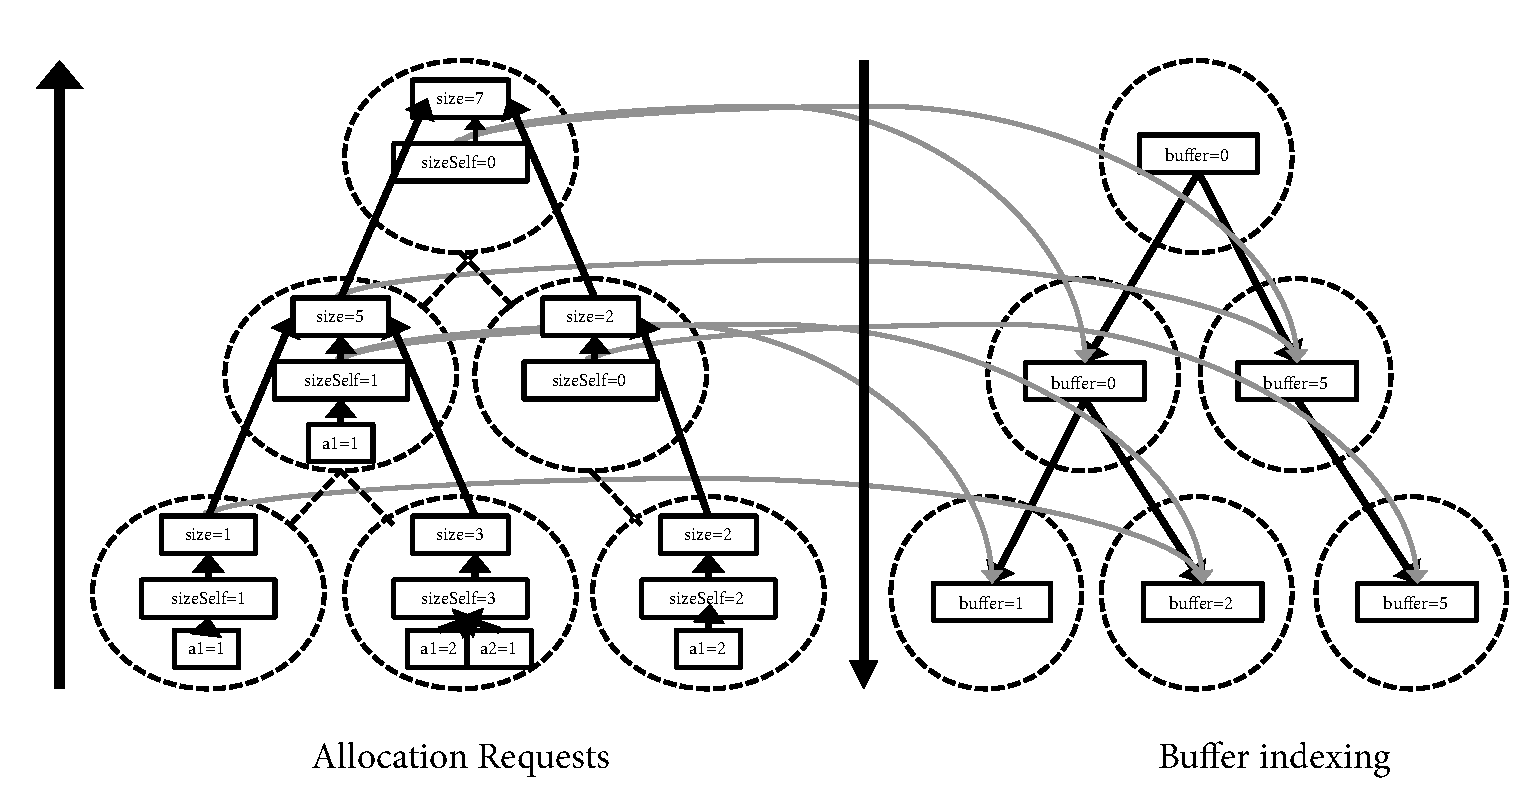
\includegraphics[trim=0 0 0 0,clip,width=1.0\columnwidth]{chapter6/macro}
\caption{\textbf{Staged parallel memory allocation as two tree traversals.} First pass is parallel bottom-up traversal computing the sum of allocation requests and the second pass is a parallel top-down traversal computing buffer indices. Lines with arrows indicate dynamic data dependencies.}
\label{fig:renderingtraversal}
\end{figure}


\subsection{Problem}
The static language of traversals is restricted, but we find that it can express important cases of typically more dynamic constructs. Prominent in our case studies, dynamic memory allocation provides significant flexibility for a language, but it is unclear how to perform it on a GPU without significant performance penalties. Our insight is that the memory allocation may be staged with parallel traversals by using a variant of prefix sum node labeling. One pass gathers  memory requests, a bulk allocation for the total amount is made, and then a scatter pass provides each node with a contiguous memory segment of it. We found manipulating memory addresses in this way to be error-prone, so we created two complementary automation techniques. First, we use our synthesizer to automatically schedule parallel memory allocation. Second, we syntactically hide the use of our optimization through a macro that automatically expands into staged dynamic memory allocation and consumption calls.

For example, we found parallel dynamic memory allocation to simplify the transition between layout and rendering. All nodes that render a circle will call some form of \code{drawCircle} in Figure~\ref{fig:stagedalloc:original}. Depending on the size of the circle, which is computed as part of the layout traversals, a different amount of memory will be allocated. Once the memory is allocated, vertices will be filled in with the correct position. The rendering engine will then connect the vertices with lines and paint them to the screen. The processing of converting the abstract shape into renderable vertices is known as tessellation. We want our system to tesselate the display objects for each node in parallel.




\subsection{Staged Parallel Memory Allocation}
We stage the use of dynamic memory into four logical phases: 
\begin{enumerate}
\item Parallel request (bottom-up tree traversal to gather )
\item Physical memory allocation
\item Parallel response (top-down tree traversal to scatter)
\item Computations that consume dynamic memory (normal parallel tree traversals)
\end{enumerate}
 The staging allows us to parallelize the request and response stages. We reuse the parallel tree traversals for them, as well as for the actual consumption. The actual allocation of physical memory in stage 2 is fast because it is a single call. Figure~\ref{fig:renderingtraversal} shows the dynamic data dependencies and two parallel tree traversals for an instance of staged parallel memory allocation.

Library functions that requires dynamic memory allocation are manually rewritten into allocation request  (Figure~\ref{fig:stagedalloc:alloc}) and memory consumption fragments (Figure~\ref{fig:stagedalloc:Render}). The transformation was not onerous to perform on our library primitives and, in the future, might be automated. 

Invocations of the original in the attribute grammar are rewritten to use the new primitives. For example, drawing two circles (Figure~\ref{fig:stagedallocClient:original}) is split into calls for allocation requests, buffer pointer manipulation, and buffer usage (Figure~\ref{fig:stagedallocClient:expanded}). The transformation increases memory consumption costs due to book keeping of allocation sizes. 

The result of our staging is three logical parallel passes, which, in practice, is merged into two parallel passes over the tree. The first pass is bottom up, similar to a prefix sum: each node computes its allocation requirements, adds that to the allocation requirements of its children,and then the process repeats for the next level of the tree. The \code{sizeSelf} and \emph{size} attributes are used for the first pass. Once the cumulative memory needs is computed, a bulk memory allocation occurs, and then a parallel top-down traversal assigns each node a memory span from \code{buffer} to \code{buffer + selfSize}. Finally, the memory can be used for actual computations through normal parallel passes. Memory use can occur immediately upon computation of the buffer index, so the last two logical stages are merged in implementation.

\subsection{Automation with Automatic Scheduling and Macros}
Manually manipulating the allocation requests and buffer pointers is error prone. We eliminated the problem through two automation techniques: automatic scheduling to enforce correct parallelization and macro expansion to encapsulate buffer manipulation.

To enforce proper parallelization, we relied upon our synthesizer to schedule the calls. If the synthesizer cannot schedule allocation calls and buffer propagation, it reports an error. Our insight is that, implicit to our staged representation, we could faithfully abstract the memory manipulations as foreign function calls. Our synthesizer simply performs its usual scheduling procedure.

To encapsulate buffer manipulation, we introduced the macro '@'.  Code that uses it is similar to code that assumes dynamic memory allocation primitives: the slight syntactic difference can be seen between Figure~\ref{fig:stagedallocClient:macro}  and Figure~\ref{fig:stagedallocClient:original}. Our macros (implemented in OMetaJS~[[CITE]]) automatically expand into the form seen in Figure~\ref{fig:stagedallocClient:expanded}. 

Our use case only required one allocation stage, but multiple may be needed.  For example, a final logging stage might be added that should run after all other computations, including rendering. However, the '@' calls described above expand to contribute to one attribute (\code{size}): no allocation is made until all of the sizes are known, which prevents making an allocation after using dynamic memory. To support multiple allocation stages, the '@' macro could be expanded to include logical group names: \code{@[render]Circle(...)} would contribute to \code{sizeRender}, \code{@[log]error(...)} to \code{sizeLog}, and \code{@[render,log]Strange(...)} to both \code{sizeRender} and \code{sizeLog}. Parallel traversals would be created for each logical name, and the synthesizer would be responsible for determining if the traversals can be merged in the final schedule and implementation.



\subsection{Evaluation}
\begin{enumerate}
\item structure split BFS  benefit for data viz and webpages
\item clustering limit study and benchmarks
\item CPU vs GPU for layout, then factor in rendering loop
\end{enumerate}
\section{Related Work}
\begin{enumerate}
\item representation The representation might be further compacted. For example, the last two arrays will have null values for Circle nodes. Even in the case of full utilization, space can be traded for time for even more aggressive compression [[CITE rinard]]
\item duane
\item trishul
\item gnu irregular array stuff
\end{enumerate}
